\documentclass[11pt]{report}
% Same style as 1-foundations/theory/preamble.tex (the course's own documents).

\usepackage[a4paper,margin=2.3cm,headheight=14pt]{geometry}
\usepackage[T1]{fontenc}
\usepackage[utf8]{inputenc}
\usepackage{lmodern}
\usepackage{microtype}
\usepackage{booktabs}
\usepackage{longtable}
\usepackage{array}
\usepackage{xcolor}
\usepackage{enumitem}
\usepackage{amssymb}
\usepackage{amsmath}
\usepackage{fancyhdr}
\usepackage{listings}
\usepackage{tikz}
\usetikzlibrary{arrows.meta,positioning,calc,fit,shapes.geometric,decorations.pathreplacing}
\usepackage[hidelinks]{hyperref}

\definecolor{warnbg}{RGB}{255,247,230}
\definecolor{warnrule}{RGB}{204,136,0}
\definecolor{newbg}{RGB}{235,245,255}
\definecolor{newrule}{RGB}{40,110,190}
\definecolor{keybg}{RGB}{237,247,237}
\definecolor{keyrule}{RGB}{50,120,60}
\definecolor{headgray}{RGB}{90,90,90}
\definecolor{codebg}{RGB}{248,248,248}

\usepackage[most]{tcolorbox}

\newtcolorbox{warnbox}[1][]{colback=warnbg,colframe=warnrule,boxrule=0.8pt,
  left=6pt,right=6pt,top=5pt,bottom=5pt,arc=1pt,#1}
\newtcolorbox{infobox}[1][]{colback=newbg,colframe=newrule,boxrule=0.8pt,
  left=6pt,right=6pt,top=5pt,bottom=5pt,arc=1pt,#1}
% "In SWEB": where the idea shows up in the course's kernel
\newtcolorbox{swebbox}[1][]{colback=newbg,colframe=newrule,boxrule=0.8pt,
  left=6pt,right=6pt,top=5pt,bottom=5pt,arc=1pt,
  title={In SWEB},fonttitle=\bfseries\small,coltitle=white,colbacktitle=newrule,#1}
% end-of-chapter summary
\newtcolorbox{keybox}[1][]{colback=keybg,colframe=keyrule,boxrule=0.8pt,
  left=6pt,right=6pt,top=5pt,bottom=5pt,arc=1pt,
  title={Key points},fonttitle=\bfseries\small,coltitle=white,colbacktitle=keyrule,#1}

\newcommand{\tbd}{\textcolor{warnrule}{\textbf{[confirm]}}}
\newcommand{\code}[1]{\texttt{#1}}
\newcommand{\file}[1]{\texttt{\small #1}}
\newcommand{\module}[1]{\textsf{module~#1}}

\setlist[itemize]{topsep=2pt,itemsep=1.5pt,parsep=0pt,leftmargin=1.3em}
\setlist[enumerate]{topsep=2pt,itemsep=1.5pt,parsep=0pt,leftmargin=1.6em}
\setlist[description]{topsep=2pt,itemsep=1.5pt,parsep=0pt,leftmargin=1.3em}

\newcolumntype{L}[1]{>{\raggedright\arraybackslash}p{#1}}

\lstset{
  language=C,
  basicstyle=\ttfamily\small,
  keywordstyle=\color{newrule}\bfseries,
  commentstyle=\color{headgray}\itshape,
  stringstyle=\color{warnrule!80!black},
  backgroundcolor=\color{codebg},
  frame=single, rulecolor=\color{black!15}, framesep=3pt,
  xleftmargin=4pt, xrightmargin=4pt, aboveskip=6pt, belowskip=4pt,
  columns=fullflexible, keepspaces=true, showstringspaces=false,
  upquote=true, tabsize=2,
  morekeywords={size_t,ssize_t,pid_t,pthread_t,pthread_mutex_t,pthread_cond_t,
                sem_t,uint8_t,uint32_t,uint64_t,bool,_Atomic,atomic_int,
                atomic_flag,__thread,_Noreturn,__asm__,volatile,pointer,uint64}
}
\lstdefinestyle{shell}{language=bash,morekeywords={},keywordstyle=\color{black}}
\lstdefinestyle{cpp}{language=C++}

\pagestyle{fancy}
\fancyhf{}
\renewcommand{\headrulewidth}{0.4pt}
\fancyhead[L]{\small\textcolor{headgray}{SWEB interview guide}}
\fancyhead[R]{\small\textcolor{headgray}{\leftmark}}
\fancyfoot[C]{\small\thepage}
\renewcommand{\chaptermark}[1]{\markboth{\thechapter\ \ #1}{}}
\fancypagestyle{plain}{\fancyhf{}\renewcommand{\headrulewidth}{0pt}\fancyfoot[C]{\small\thepage}}

\renewcommand{\arraystretch}{1.25}
\setlength{\parskip}{3pt}
\setlength{\parindent}{0pt}
\setlength{\emergencystretch}{3em}   % fewer overfull lines with long \code words

% guide additions
\newtcolorbox{lockbox}[1][]{colback=warnbg,colframe=warnrule,boxrule=0.8pt,
  left=6pt,right=6pt,top=5pt,bottom=5pt,arc=1pt,
  title={Locking},fonttitle=\bfseries\small,coltitle=white,colbacktitle=warnrule,#1}
\newtcolorbox{trapbox}[1][]{colback=warnbg,colframe=warnrule,boxrule=0.8pt,
  left=6pt,right=6pt,top=5pt,bottom=5pt,arc=1pt,
  title={Trap},fonttitle=\bfseries\small,coltitle=white,colbacktitle=warnrule,#1}
\lstset{morekeywords={ScopeLock,Mutex,Condition,SpinLock,ArchThreadRegisters,ArchMemoryMapping},
  breaklines=true, breakatwhitespace=true, postbreak=\mbox{\textcolor{headgray}{$\hookrightarrow$}\space}}
\renewcommand{\file}[1]{\texttt{#1}}   % inherit the size of the surrounding text (tables use \footnotesize)


\begin{document}

\begin{titlepage}
  \centering
  \vspace*{3cm}
  {\Huge\bfseries SWEB Interview Guide\par}
  \vspace{0.6cm}
  {\Large What happens where, how to change it --- and how to lock it\par}
  \vspace{2cm}
  {\large Theory for the live-coding part of the Abgabegespräche A0, A1, A2\par}
  \vfill
  \begin{infobox}
  Companion to \file{preparation/2-ag-interviews/}: the examples (\code{exNN}), the tasks
  (\code{a0/}, \code{a1/}, \code{a2/}) and their solutions refer to the sections here, and
  the sections point back to them. Every claim about SWEB in this guide was checked against
  the code (upstream \code{f6fcb2ab}) and, where it matters, by running it.
  \end{infobox}
  \vspace{1cm}
  {\small A self-study companion for Operating Systems at TU Graz,\\ winter semester 2026/27 --- not official course material\par}
\end{titlepage}

\tableofcontents

\chapter{The interview}
\label{ch:interview}

\section{What happens}

In every Abgabegespräch each group member gets a small task, comparable in difficulty to
the assignment tasks, and implements it live in the group's SWEB while the tutor watches
(official rules page). You also explain code --- usually a snippet of your own
implementation, often while you implement. If you are slow or cannot explain or
implement, you get an \emph{individual} deduction on the assignment's points. The tutor
stops you as soon as it is clear that you deserve the points: you do not have to finish a
polished solution, you have to show that you \emph{know where things happen and how to
change them correctly}.

Students' reports (see \file{a0/README.md}) agree on three things: the tasks are about
\textbf{syscalls}, the \textbf{page fault handler} and \textbf{page mappings}, threads and
\textbf{registers}; knowing your way around the code matters more than any single
algorithm; and the most common reason for deductions is \textbf{locking} --- missing or
wrong (chapter~\ref{ch:locking}).

\section{A strategy for the 30 minutes}

\begin{enumerate}
\item \textbf{Restate the task} in one sentence and ask about the edge cases you see
  (``what should happen if the pointer is invalid?''). Tutors expect questions.
\item \textbf{Say where it happens.} ``A segfault ends up in
  \code{PageFaultHandler::handlePageFault}, and for addresses without a segment in
  \code{Loader::loadPage} --- I'll hook in there.'' Chapter~\ref{ch:map} is the map for this step.
\item \textbf{List the pieces} before typing: syscall (6 places), per-process state (where?),
  page-fault branch, libc wrapper, test. Chapter~\ref{ch:recipes} has the checklists.
\item \textbf{Write the minimal correct version.} No refactoring of existing code, no
  generality nobody asked for.
\item \textbf{Locking pass.} For every piece of shared state you touched: which lock, where
  taken, where released, could anything run in between? Say it out loud.
\item \textbf{Test} with a tiny program in \file{userspace/tests/} --- and show the error path.
\end{enumerate}

\begin{infobox}[title=\textbf{Talking while coding}]
Practise narrating: what you look for, why this file, why this lock. It makes the tutor
see your understanding even when you have to look something up, and it keeps you from
silently typing yourself into a corner. The tasks' ``questions a tutor might ask'' are
there for this.
\end{infobox}

\section{How to use this course}

\begin{description}
\item[Examples] (\file{examples/}) --- one mechanism each, complete and tested; read the
  patch, apply it, run it. They are your reference when a task needs ``that thing with the
  ident mapping''.
\item[Tasks] (\file{a0/}, \file{a1/}, \file{a2/}) --- task cards in the tutors' format, a
  test program, hints behind fold-outs, questions. Time-box them.
\item[Solutions] (\file{solutions/}) --- patch plus \file{NOTES.md}. Read the \emph{Locking}
  and \emph{Pitfalls} sections even when your version works.
\item[Tools] --- you work in a separate training copy of SWEB, \file{repos/sweb-ag}, one git
  branch per task (created once with \code{task.sh setup}). \code{tools/task.sh} does the bookkeeping:
  \code{task.sh start a0-01} (fresh branch from the right base, tests copied in),
  \code{task.sh test} (build + run the tests without a window, with leak check),
  \code{task.sh run} / \code{kvm} / \code{debug} + \code{gdb} (exactly like \code{sweb-practise}),
  \code{task.sh reset a0-01} or \code{reset a1} (start over --- your attempt is kept in a
  \code{backup/} branch), \code{task.sh solution a0-01} and \code{task.sh diff a0-01}.
\end{description}

\chapter{The map: what happens where}
\label{ch:map}

This chapter answers ``which file do I have to touch?''. Read it once completely, then
use the tables as a lookup during practice.

\section{The source tree --- the parts you touch}

\begin{center}
\footnotesize
\begin{tabular}{L{7.0cm}L{8.6cm}}
\toprule
\textbf{Path} & \textbf{What lives there} \\
\midrule
\file{common/include/kernel/syscall-definitions.h} & syscall numbers (\code{sc\_...}) --- included by kernel \emph{and} libc \\
\file{common/source/kernel/Syscall.cpp} & \code{syscallException}: the big switch; all syscall implementations \\
\file{common/source/mm/PageFaultHandler.cpp} & \code{enterPageFault}, \code{checkPageFaultIsValid}, \code{handlePageFault} \\
\file{common/source/kernel/Loader.cpp} & the ELF binary of a process, \code{loadPage} (lazy loading), owns the address space \code{arch\_memory\_} \\
\file{common/source/kernel/UserProcess.cpp} & process start: loader, first stack page, user registers \\
\file{common/source/kernel/Thread.cpp} & \code{Thread}: kernel stack, registers, state, \code{kill()} \\
\file{common/source/kernel/Scheduler.cpp} & thread list, \code{schedule()} (round robin), \code{yield}, \code{sleep}/\code{wake}, cleanup \\
\file{common/source/kernel/ProcessRegistry.cpp} & starts the programs of \code{user\_progs.h} (the shell) and \code{createprocess} \\
\file{common/source/kernel/}\newline\file{\{Mutex,SpinLock,Condition,ScopeLock,Lock\}.cpp} & locks, with deadlock and misuse checks \\
\file{common/source/kernel/main.cpp} & \code{startup()}: boot order; create kernel-wide objects here \\
\file{common/source/mm/PageManager.cpp} & physical pages: \code{allocPPN} (zeroed), \code{freePPN}, free/total counts \\
\file{common/source/mm/KernelMemoryManager.cpp} & the kernel heap behind \code{new}/\code{delete} \\
\file{common/source/console/Console.cpp} & \code{handleKey}: F-keys (F9--F12 debug output, Shift+Fn terminal switch) \\
\file{common/source/fs/BDManager.cpp},\newline\file{BDVirtualDevice.cpp} & block devices: \code{idea0}, \code{idea1} (\file{/usr}), \code{idea2} (swap partition) \\
\file{common/include/console/debug.h} & debug flags: \code{debug(FLAG, ...)} on/off per category \\
\midrule
\file{arch/x86/64/source/InterruptUtils.cpp} & C entry of every interrupt: \code{syscallHandler}, \code{pageFaultHandler}, \code{errorHandler}, timer \code{irqHandler\_0}, keyboard \code{irqHandler\_1} \\
\file{arch/x86/64/source/arch\_interrupts.S} & the assembly stubs: save registers, call the C handler, \code{iretq} \\
\file{arch/x86/64/source/ArchMemory.cpp} & page tables: \code{mapPage}, \code{unmapPage}, \code{resolveMapping}, \code{checkAddressValid}, \code{flushTlb} \\
\file{arch/x86/64/include/paging-definitions.h} & the page-table entry bit fields (\code{PageTableEntry}: present, writeable, user\_access, dirty, ignored\_*, execution\_disabled) \\
\file{arch/x86/64/source/ArchThreads.cpp} & \code{createUserRegisters}, \code{createKernelRegisters}, \code{setAddressSpace}, atomics \\
\file{arch/x86/64/include/ArchThreads.h} & \code{struct ArchThreadRegisters} (rip, rsp, rax, rdi, \ldots, cr3) \\
\file{arch/x86/64/include/offsets.h} & \code{USER\_BREAK}, \code{KERNEL\_START}, \code{IDENT\_MAPPING\_START} \\
\midrule
\file{arch/x86/64/userspace/syscalls.c} & \code{\_\_syscall}: \code{int \$0x80}, number in \code{rax}, args in \code{rbx, rcx, rdx, rsi, rdi} \\
\file{userspace/libc/src/*.c},\newline\file{userspace/libc/include/*.h} & the libc: \code{nonstd.c} (SWEB extras), \code{pthread.c}, \code{stdlib.c} (\code{malloc} is a stub!), \ldots \\
\file{userspace/tests/*.c} & one program per file, \code{name.c} $\to$ \code{name.sweb} on the disk image \\
\bottomrule
\end{tabular}
\end{center}

\section{When X happens --- the call chains}

\begin{center}
\small
\begin{longtable}{L{2.6cm}L{12.2cm}}
\toprule
\textbf{Event} & \textbf{Chain (file)} \\
\midrule
\endhead
System call &
user: libc wrapper (\file{nonstd.c}) $\to$ \code{\_\_syscall} (\file{arch/x86/64/userspace/syscalls.c}): \code{int \$0x80}
$\to$ \code{arch\_syscallHandler} (\file{arch\_interrupts.S}): save user registers into \code{currentThread->user\_registers\_}
$\to$ \code{syscallHandler} (\file{InterruptUtils.cpp}): \code{switch\_to\_userspace\_ = 0}, interrupts \textbf{on}
$\to$ \code{Syscall::syscallException(rax, rbx, rcx, rdx, rsi, rdi)} (\file{Syscall.cpp})
$\to$ return value into \code{user\_registers\_->rax}, \code{arch\_contextSwitch()} loads the user registers. \\
\addlinespace
Page fault (\#PF, vector 14) &
\code{arch\_pageFaultHandler} (asm: \code{cr2} = address, error code from the stack)
$\to$ \code{pageFaultHandler(address, error)} (\file{InterruptUtils.cpp}): decodes present / write / user / fetch
$\to$ \code{PageFaultHandler::enterPageFault} (kernel registers, interrupts \textbf{on})
$\to$ \code{handlePageFault}: \code{checkPageFaultIsValid}? no: backtrace + \code{Syscall::exit(9999)};
yes: \code{loader\_->loadPage(address)} (\file{Loader.cpp}): no segment covers it $\to$ \code{Syscall::exit(666)}
$\to$ back: the faulting instruction is executed again. \\
\addlinespace
CPU exception (div by 0, \#GP, \ldots) &
\code{errorHandler} (\file{InterruptUtils.cpp}): prints the error and registers; user thread $\to$ \code{Syscall::exit(888)}, kernel thread $\to$ \code{kill()}. \\
\addlinespace
Timer tick (IRQ 0) &
\code{irqHandler\_0}: \code{Scheduler::incTicks()}, \code{Scheduler::schedule()} (picks the next schedulable thread, sets \code{currentThreadRegisters}), \code{arch\_contextSwitch()} --- a thread can lose the CPU \textbf{between any two instructions} when interrupts are on. \\
\addlinespace
\code{yield()} &
\code{Scheduler::yield} $\to$ \code{int \$65} $\to$ \code{irqHandler\_65}: \code{schedule()} + context switch. \\
\addlinespace
Key press &
IRQ 1 $\to$ \code{KeyboardManager::serviceIRQ} (\file{arch/x86/common}) queues the key $\to$ the \textbf{Console kernel thread} (\code{Console::Run}) takes it: printable $\to$ terminal; F-keys $\to$ \code{Console::handleKey}. \\
\addlinespace
Program start &
boot: \code{startup()} (\file{main.cpp}) adds the \code{ProcessRegistry} thread $\to$ \code{Run()} mounts \file{/usr}, \code{createProcess(path)} for each entry of \code{user\_progs.h} (the shell).
Shell runs \code{foo.sweb} $\to$ \code{createprocess} syscall $\to$ \code{ProcessRegistry::createProcess} $\to$ \code{new UserProcess(path)}:
open file, \code{new Loader(fd)}, read ELF headers, map \textbf{one} stack page at \code{USER\_BREAK - PAGE\_SIZE},
\code{createUserRegisters(rip = ELF entry, rsp = USER\_BREAK - 8)}, \code{setAddressSpace} $\to$ \code{Scheduler::addNewThread}.
The first schedule loads the user registers: the program starts in \code{\_start} (\file{nonstd.c}) $\to$ \code{main}. \\
\addlinespace
Kernel thread start &
\code{new MyThread} (\code{Thread(..., KERNEL\_THREAD)}: kernel registers with \code{rip = threadStartHack}) $\to$ \code{addNewThread} $\to$ first schedule: \code{threadStartHack} $\to$ \code{Run()} $\to$ \code{kill()}. \\
\addlinespace
Thread / process end &
\code{exit()} $\to$ \code{Syscall::exit} $\to$ \code{currentThread->kill()}: state \code{ToBeDestroyed}, \code{yield()}, never returns.
The \textbf{CleanupThread} (\code{cleanupDeadThreads}) removes it from the list and \code{delete}s it $\to$ \code{\textasciitilde UserProcess}: \code{delete loader\_} $\to$ \code{\textasciitilde ArchMemory} frees every user page and page table; \code{ProcessRegistry::processExit}. \\
\addlinespace
Disk I/O &
\code{BDVirtualDevice::readData/writeData} $\to$ \code{BDRequest} into the driver's queue $\to$ the thread yields until the IDE interrupt (IRQ 14/15) marks it done. \\
\addlinespace
Kernel \code{new} &
\code{KernelMemoryManager} (own lock), pages come from the \code{PageManager}. \\
\bottomrule
\end{longtable}
\end{center}

\section{The two paths you will change most}

\begin{center}
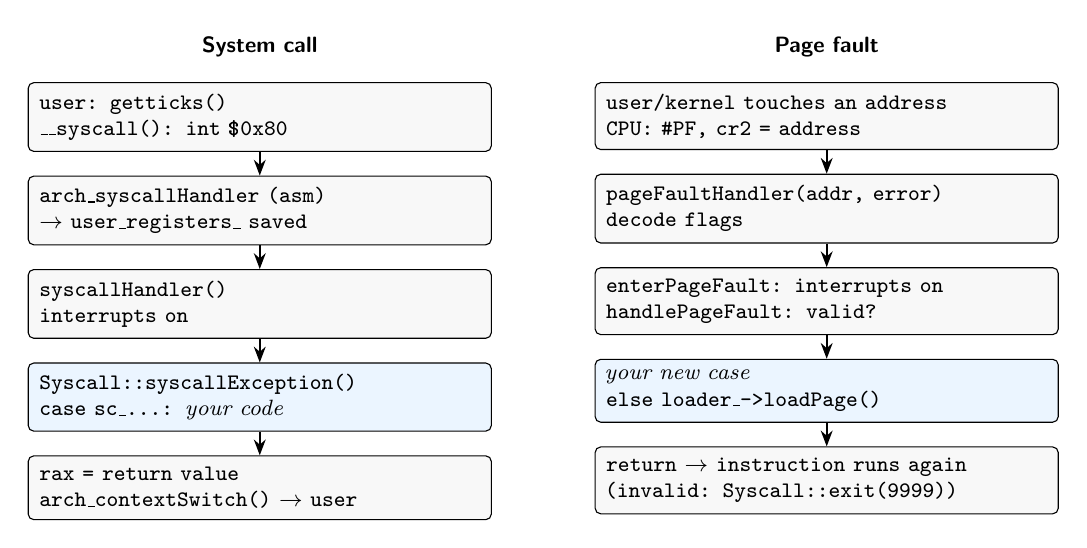
\begin{tikzpicture}[
  box/.style={draw, rounded corners=2pt, fill=codebg, align=left, font=\footnotesize\ttfamily,
              inner sep=4pt, text width=5.6cm},
  lab/.style={font=\footnotesize\sffamily\bfseries},
  arr/.style={-{Stealth[length=2mm]}, thick}]
  \node[lab] (s0) at (0,0) {System call};
  \node[box, below=2mm of s0] (s1) {user: getticks() \\ \_\_syscall(): int \$0x80};
  \node[box, below=3mm of s1] (s2) {arch\_syscallHandler (asm) \\ $\to$ user\_registers\_ saved};
  \node[box, below=3mm of s2] (s3) {syscallHandler() \\ interrupts on};
  \node[box, below=3mm of s3, fill=newbg] (s4) {Syscall::syscallException() \\ case sc\_...: \textrm{\itshape your code}};
  \node[box, below=3mm of s4] (s5) {rax = return value \\ arch\_contextSwitch() $\to$ user};
  \draw[arr] (s1) -- (s2); \draw[arr] (s2) -- (s3); \draw[arr] (s3) -- (s4); \draw[arr] (s4) -- (s5);

  \node[lab] (p0) at (7.2,0) {Page fault};
  \node[box, below=2mm of p0] (p1) {user/kernel touches an address \\ CPU: \#PF, cr2 = address};
  \node[box, below=3mm of p1] (p2) {pageFaultHandler(addr, error) \\ decode flags};
  \node[box, below=3mm of p2] (p3) {enterPageFault: interrupts on \\ handlePageFault: valid?};
  \node[box, below=3mm of p3, fill=newbg] (p4) {\textrm{\itshape your new case} \\ else loader\_->loadPage()};
  \node[box, below=3mm of p4] (p5) {return $\to$ instruction runs again \\ (invalid: Syscall::exit(9999))};
  \draw[arr] (p1) -- (p2); \draw[arr] (p2) -- (p3); \draw[arr] (p3) -- (p4); \draw[arr] (p4) -- (p5);
\end{tikzpicture}
\end{center}

Both run \textbf{in the context of the thread that caused them}: \code{currentThread} is that
thread, its page tables are active, \code{currentThread->user\_registers\_} holds its user
state, and interrupts are enabled --- you may take Mutexes, allocate, sleep, do disk I/O.
That is not true in the timer interrupt, in \code{schedule()}, or in the keyboard IRQ.

\section{Who owns what}

\begin{center}
\small
\begin{tabular}{L{3.4cm}L{11.4cm}}
\toprule
\textbf{Object} & \textbf{Owns / knows} \\
\midrule
\code{Thread} & kernel stack (\code{kernel\_stack\_}, 8 KiB), \code{kernel\_registers\_}, \code{user\_registers\_} (user threads), \code{switch\_to\_userspace\_}, state (\code{Running}/\code{Sleeping}/\code{ToBeDestroyed}), \code{loader\_}, terminal, working dir \\
\code{UserProcess} & base SWEB: \emph{is} the one thread of a process (\code{: public Thread}); owns the \code{Loader} and the file descriptor of the binary \\
\code{Loader} & the binary (\code{fd\_}, ELF header, \code{phdrs\_}), \code{program\_binary\_lock\_}, and \code{arch\_memory\_} --- \textbf{the address space} \\
\code{ArchMemory} & the PML4 of one address space (\code{page\_map\_level\_4\_}) and everything below it \\
\code{PageManager} & which physical pages are free (bitmap), SpinLock \\
\code{Scheduler} & the list of all threads; ticks \\
\code{ProcessRegistry} & the number of running processes; starting programs \\
\bottomrule
\end{tabular}
\end{center}

In base SWEB, \textbf{per-process state belongs into the \code{Loader}} (the only per-process
object every thread can reach: \code{currentThread->loader\_}). In the team repo it belongs
into \code{UserProcess} (chapter~\ref{ch:team}).

\section{The address space}

\begin{center}
\small
\begin{tabular}{L{5.2cm}L{9.6cm}}
\toprule
\textbf{Address} & \textbf{What} \\
\midrule
\code{0x0 -- 0xFFF} & never mapped: null pointer accesses fault \\
\code{0x400000}, \code{0x8000000}\ldots & the program: \code{.text} (R E) at \code{0x8000000}, \code{.rodata} (R), \code{.data}/\code{.bss} (RW) --- \code{readelf -lW prog.sweb} \\
\code{0x5000\,0000\,0000} etc. & free: this course's tasks put regions here (alloc region, heap at \code{0x6000\ldots}, scratch \code{0x7000\ldots}) \\
\code{USER\_BREAK - 4096} & the main thread's stack page (only this one is mapped at start) \\
\code{USER\_BREAK} = \code{0x8000\,0000\,0000} & end of user space (lower canonical half) \\
\code{0x8000\ldots{} -- 0xFFFF\,7FFF\ldots} & non-canonical: any access is a \#GP \\
\code{KERNEL\_START} = \code{0xFFFF\,8000\,0000\,0000} & kernel half: identical in every PML4 \\
\code{IDENT\_MAPPING\_START} = \code{0xFFFF\,F000\,0000\,0000} & \textbf{ident mapping}: all physical memory, \code{getIdentAddressOfPPN(ppn)} \\
\code{0xFFFF\,FFFF\,8000\,0000} & the kernel image (code, data, the threads' kernel stacks) \\
\bottomrule
\end{tabular}
\end{center}

\begin{swebbox}
Because the kernel half is the same in every address space and the kernel runs with the
current process's \code{cr3}, a syscall can read and write that process's user memory
directly through the user pointer. Through the \emph{ident mapping} the kernel can read and
write \emph{any} physical page, including pages of other processes and pages not mapped
anywhere --- that is how page contents are prepared (A0-04), copied (fork, A1), and written
to disk (swap, A2).
\end{swebbox}

\section{Registers: user, kernel, current}

\code{struct ArchThreadRegisters} (\file{arch/x86/64/include/ArchThreads.h}) holds a full
register set: \code{rip, cs, rflags, rax, rcx, rdx, rbx, rsp, rbp, rsi, rdi, r8--r15,
ds, es, fs, gs, ss, rsp0, cr3, fpu}. A user thread has two sets:

\begin{description}
\item[\code{user\_registers\_}] the user-mode state. Saved on every entry into the kernel
  from user mode (syscall, page fault, interrupt). \textbf{While you are in a syscall or a
  user page fault, it is exactly the state the user thread will continue with} ---
  change it and the thread continues differently (ex05, A0-06, A0-07).
\item[\code{kernel\_registers\_}] the kernel-mode state, saved when the thread is
  interrupted \emph{in} the kernel.
\end{description}

\code{currentThreadRegisters} points to the set that the next \code{arch\_contextSwitch()}
loads; \code{switch\_to\_userspace\_} says which one it is. The syscall and page-fault
entries set it to the kernel set while the kernel works, and back to the user set before
returning.

Calling convention (System V AMD64): arguments in \code{rdi, rsi, rdx, rcx, r8, r9}, result
in \code{rax}; at function entry \code{rsp \% 16 == 8}; the 128 bytes below \code{rsp} are the
\textbf{red zone} of the running function. SWEB's syscall ABI is different: number in
\code{rax}, arguments in \code{rbx, rcx, rdx, rsi, rdi}.

\chapter{Recipes}
\label{ch:recipes}

Checklists and code templates for every kind of change the tasks need. Each recipe names
the example that shows it working.

\section{Add a syscall (ex01)}
\label{sec:syscall}

\begin{center}
\footnotesize
\begin{tabular}{cL{6.6cm}L{8.2cm}}
\toprule
& \textbf{File} & \textbf{Add} \\
\midrule
1 & \file{common/include/kernel/syscall-definitions.h} & \code{\#define sc\_foo 1500} \\
2 & \file{common/include/kernel/Syscall.h} & \code{static size\_t foo(size\_t a, size\_t b);} \\
3 & \file{common/source/kernel/Syscall.cpp} & \code{case sc\_foo: return\_value = foo(arg1, arg2); break;} \\
4 & \file{common/source/kernel/Syscall.cpp} & the implementation \\
5 & \file{userspace/libc/include/nonstd.h} (or \code{pthread.h}, \ldots) & \code{extern int foo(int a, void* b);} \\
6 & \file{userspace/libc/src/nonstd.c} & \code{return \_\_syscall(sc\_foo, a, (size\_t) b, 0x00, 0x00, 0x00);} \\
\bottomrule
\end{tabular}
\end{center}

\begin{lstlisting}[style=cpp]
size_t Syscall::foo(size_t a, size_t user_ptr)
{
  if (user_ptr == 0 || user_ptr >= USER_BREAK - sizeof(Thing))  // check first
    return (size_t) -1;
  Thing copy = ...;                                            // work on kernel data
  *(Thing*) user_ptr = copy;                                    // one copy to user space at the end
  return 0;
}
\end{lstlisting}

\begin{trapbox}
\begin{itemize}
\item \code{return -1U;} is \code{0xFFFFFFFF} --- user space sees 4294967295. Use \code{(size\_t) -1}.
\item Forgotten \code{break;} $\to$ falls through into the next case.
\item \code{-Werror}: an unused parameter, a missing include, initializers out of
  declaration order (\code{-Werror=reorder}) all stop the build.
\item \file{nonstd.h} does not include \file{types.h} $\to$ \code{unknown type name 'size\_t'}.
\item At most 5 arguments. More: pass a pointer to a struct or array (A1 ``15-argument syscall'').
\item A new test \code{.c} needs cmake to run again (\code{run\_test.sh} does it) --- and a
  second \code{make}: a parallel build may copy the programs to the disk image before they
  are built (\code{loading /usr/shell.sweb failed}).
\end{itemize}
\end{trapbox}

\section{User pointers}
\label{sec:userptr}

\begin{enumerate}
\item \textbf{Check the whole range} below \code{USER\_BREAK}, overflow-safe:
  \code{p == 0 || p >= USER\_BREAK - size} $\to$ reject. (\code{p + size > USER\_BREAK} can wrap around.)
\item \textbf{Copy in, then check, then use.} Another thread of the process can change user
  memory between your check and your use (TOCTOU). Copy into a kernel variable first,
  validate the copy (A0-09: function pointers).
\item \textbf{Write results back at the end}, after all locks are released: a user page that
  is not mapped yet page-faults --- in kernel mode, on a user address. That is legal (it is
  loaded like a normal fault), but it must not happen while you hold a lock, and if no
  segment covers the address the process is killed right there (order your side effects:
  A0-08 ``touch the id pointer first'').
\item Never hand a user pointer to a driver or keep it for later: copy into kernel memory.
\item \textbf{Strings have no known length} --- there is no range to check up front. Copy byte by
  byte into a bounded kernel buffer, check \emph{each} address against \code{USER\_BREAK} before
  reading it, stop at the NUL or the limit, write the NUL yourself (\code{strncpy} does not when
  the source is long). Read user memory directly, not via \code{checkAddressValid}: that one
  calls a page ``unmapped'' that is merely not loaded yet (ex11, A0-11).
\end{enumerate}

\section{Physical pages and mappings (ex02, ex04)}
\label{sec:mapping}

\begin{center}
\footnotesize
\begin{tabular}{L{6.6cm}L{8.8cm}}
\toprule
\textbf{Call} & \textbf{Does} \\
\midrule
\code{PageManager::instance()->allocPPN()} & a free physical page, \textbf{zeroed}; asserts when memory is full \\
\code{PageManager::instance()->freePPN(ppn)} & gives it back (fills it with \code{0xFF}: use-after-free is detected) \\
\code{ArchMemory::getIdentAddressOfPPN(ppn)} & kernel address of that page --- valid in every address space \\
\code{arch\_memory\_.mapPage(vpn, ppn, user)} & maps \textbf{writable}; \code{user = 1}: user may access; \code{false} if vpn already mapped (caller keeps \code{ppn}); allocates page tables on the way \\
\code{arch\_memory\_.unmapPage(vpn)} & clears the entry, \textbf{frees the physical page}, frees empty page tables; asserts if not mapped; \textbf{no TLB flush} \\
\code{arch\_memory\_.resolveMapping(vpn)} & \code{ArchMemoryMapping m}: \code{m.pt[m.pti]} is the PTE, \code{m.page\_ppn}, \code{m.page\_size} (\code{PAGE\_SIZE} iff a 4 KiB page is mapped; \code{m.pt} is \code{nullptr} if there is no page table) \\
\code{arch\_memory\_.checkAddressValid(addr)} & ident address of the byte \code{addr} if mapped, else 0 --- write user memory without risking a fault \\
\code{ArchMemory::flushTlb()} & reload \code{cr3}: forget cached translations \\
\bottomrule
\end{tabular}
\end{center}

\code{vpn} and \code{ppn} are \textbf{page numbers} (\code{address / PAGE\_SIZE}), not addresses.
\textbf{One frame, one mapping:} \code{\textasciitilde ArchMemory} frees every present user page
at exit. A frame you map a second time (an alias, a shared page) must be unmapped
\emph{without} freeing first (\code{unmapPage(vpn, false)}), or it is freed twice: kernel panic
\code{"Double free PPN"} (ex12, A0-12, A1-10).

\begin{lstlisting}[style=cpp]
// map a fresh page (outside the lock: allocate; inside: map)
size_t ppn = PageManager::instance()->allocPPN();
loader->arch_memory_lock_.acquire();
bool mapped = loader->arch_memory_.mapPage(vpn, ppn, 1);
if (mapped && read_only)
{
  ArchMemoryMapping m = loader->arch_memory_.resolveMapping(vpn);
  m.pt[m.pti].writeable = 0;            // same critical section as mapPage
}
loader->arch_memory_lock_.release();
if (!mapped)
  PageManager::instance()->freePPN(ppn); // someone else mapped it first

// unmap
loader->arch_memory_lock_.acquire();
if (loader->arch_memory_.resolveMapping(vpn).page_size)
  loader->arch_memory_.unmapPage(vpn);   // frees the ppn - don't free it again
ArchMemory::flushTlb();
loader->arch_memory_lock_.release();
\end{lstlisting}

\textbf{TLB rule:} after \emph{removing} rights (unmap, read-only, NX, swap out) flush the TLB;
after \emph{adding} rights (map a non-present page, make writable) you need not --- a stale,
weaker entry just causes one more page fault that finds everything in order.

\textbf{The page-table entry} (\code{PageTableEntry}, \file{paging-definitions.h}):
\code{present, writeable, user\_access, write\_through, cache\_disabled, accessed, dirty,
size, global, ignored\_2 (3 bits), page\_ppn (28 bits), reserved\_1, ignored\_1 (11 bits),
execution\_disabled}. The CPU sets \code{accessed} on every access and \code{dirty} on every
write. When \code{present == 0}, the CPU ignores \emph{all} other bits --- you may store your
own information there (A2: the swap slot). \code{execution\_disabled} (NX) works: SWEB enables
\code{EFER.NXE} at boot.

\textbf{Walking all page tables} (A0-01, A2 ``all pages of a process''): copy the loop of
\code{ArchMemory::\textasciitilde ArchMemory()} --- four nested loops over the present
entries, PML4 index \code{0 .. 255} only (user half).

\section{A new page fault case (ex03)}
\label{sec:pagefault}

\begin{itemize}
\item \textbf{Where:} in \code{PageFaultHandler::handlePageFault}, inside
  \code{if (checkPageFaultIsValid(...))}, \emph{before} \code{loader\_->loadPage}. Only there
  you know the fault is a non-present user address.
\item \textbf{Flags} available: \code{address}, \code{user} (fault in user mode),
  \code{present} (page was present: protection violation), \code{writing},
  \code{fetch} (instruction fetch), \code{switch\_to\_us}.
\item Faults with \code{present == 1} never reach the valid branch: \code{checkPageFaultIsValid}
  rejects them. A protection case (copy-on-write, A2) needs a branch \emph{before} that check.
\item The ``kill'' exits: 9999 invalid fault (page fault handler), 666 no segment
  (\code{Loader::loadPage}), 999 file read failed, 888 CPU exception.
\item Returning without fixing the cause $\to$ the same fault again, forever.
\end{itemize}

\section{Changing the user registers (ex05)}
\label{sec:registers}

Allowed while handling a syscall or a page fault of that thread (its
\code{user\_registers\_} are saved and will be loaded on return), or for a thread that is
not scheduled (not yet added, or sleeping).

\begin{lstlisting}[style=cpp]
ArchThreadRegisters* regs = currentThread->user_registers_;
size_t rsp = ((regs->rsp - 128) & ~0xFULL) - sizeof(size_t); // red zone, align, ret slot
pointer slot = loader->arch_memory_.checkAddressValid(rsp);  // under the page-table lock
if (!slot) { /* no usable stack */ }
*(size_t*) slot = return_address;   // e.g. regs->rip (continue after the syscall) or 0
regs->rsp = rsp;
regs->rip = function;
regs->rdi = first_argument;         // rsi, rdx, rcx, r8, r9 for more
\end{lstlisting}

The syscall's own return value still goes into \code{rax} afterwards. Why the red zone matters:
\code{objdump -d prog.sweb} $\to$ \code{<\_\_syscall>} keeps its locals at \code{-0x10(\%rbp)
... -0x38(\%rbp)} while \code{rsp = rbp - 8} --- \emph{below} \code{rsp}.

\section{Threads (ex06, A0-08)}
\label{sec:threads}

\textbf{A user thread} = same \code{loader\_} (address space) + own user stack + own
registers + an entry in the scheduler:

\begin{lstlisting}[style=cpp]
class UserThread : public Thread { ... };          // Thread(..., Thread::USER_THREAD)
loader_ = process->loader_;                         // shared address space
/* map stack pages under the page-table lock */
ArchThreads::createUserRegisters(user_registers_, (void*) entry,
                                 (void*) (stack_top - sizeof(pointer)), getKernelStackStartPointer());
user_registers_->rdi = ...; user_registers_->rsi = ...;
ArchThreads::setAddressSpace(this, loader_->arch_memory_);
// later, when everything is set up:
Scheduler::instance()->addNewThread(thread);
\end{lstlisting}

\textbf{A kernel thread}: subclass \code{Thread} with \code{KERNEL\_THREAD}, implement
\code{Run()}, \code{new} it, \code{addNewThread}. When \code{Run()} returns, it is killed
and the CleanupThread deletes it --- never delete a thread yourself, never put one on
the stack.

\textbf{Ending a thread}: \code{currentThread->kill()} --- state \code{ToBeDestroyed}, never
returns. The object lives on until the CleanupThread deletes it: \textbf{destructors run in
the CleanupThread}, when the thread can never run again --- the right place to free its
stack. Another thread cannot be killed directly ``from outside'' safely: set a flag that it
checks (A1 \code{pthread\_cancel}).

\section{Waiting for something}
\label{sec:waiting}

\begin{lstlisting}[style=cpp]
// waiter                                   // the one who makes it true
lock.acquire();                             lock.acquire();
while (!condition_is_true)                  condition_is_true = true;
  condition_variable.wait();                condition_variable.signal();   // or broadcast()
/* use the state, still locked */           lock.release();
lock.release();
\end{lstlisting}

\begin{itemize}
\item \code{Condition(\&mutex, "name")}; \code{wait()} releases the mutex while sleeping and
  re-acquires it; SWEB \textbf{asserts that you hold no other lock} while waiting.
\item \code{signal()} wakes one waiter, \code{broadcast()} all (barriers, ``all threads done'').
\item \code{Scheduler::sleep()} / \code{wake(thread)} are the low-level primitives the locks are
  built on --- using them directly is easy to get wrong (lost wake-ups); prefer a Condition.
\item A \code{while (!x) yield();} loop is \emph{busy waiting}: acceptable for a quick test,
  not for a solution the tutor should accept (``join must sleep, not spin'').
\end{itemize}

\section{From another context into a process (ex07)}

Key presses are handled in the Console kernel thread, the timer in an interrupt --- neither
runs in the target process's context. Set a flag there (\code{ArchThreads::testSetLock(flag, 1)}
is an atomic exchange; \code{atomic\_add}, \code{atomic\_set} exist too) and let the target
do the work at a safe point in its own context (top of \code{syscallException}, page fault
handler, or a kernel thread you wake).

\section{Disk (ex08)}

\code{BDManager::getInstance()->getDeviceByName("idea2")} $\to$
\code{readData(offset, size, kernel\_buffer)} / \code{writeData(...)}: offset and size in
bytes, multiples of \code{getBlockSize()} (512); returns size or -1; \textbf{blocks} (yields)
until done --- interrupts on, no SpinLock held. \code{run\_test.sh} boots with a throw-away
copy of the disk (\code{-snapshot}).

\section{Kernel-wide objects}

\textbf{SWEB never runs constructors of global or static objects.} A global
\code{Mutex lock("x");} is zeroed memory and asserts on first use. Create such objects with
\code{new} in \code{startup()} (\file{main.cpp}) before the threads that use them exist, or
make them members of a singleton that is created at boot.

\section{Testing traps}
\label{sec:testing}

\begin{itemize}
\item \textbf{The timer runs at 18.2\,Hz} (\code{IRQ0\_TIMER\_FREQUENCY} is 0, the PIT keeps its
  default divisor 65536): one tick is 55\,ms. A round of \code{sched\_yield} passes the IdleThread,
  which halts until the next tick --- \textbf{300 yields take about 16 seconds}. Loops that yield
  look like hangs. Compute instead, or sleep on a Condition.
\item QEMU is fast: a busy loop of millions of iterations finishes within one 55\,ms time slice.
  To get a deterministic order between threads, let them yield a different number of times.
\item Lazy loading: a page of \code{.bss} or \code{.data} that was never touched has no frame yet
  (\code{vtop} $\to$ -1, \code{mprotect} fails, statistics are smaller than expected).
\item The disk image keeps every program ever built into it; after many tasks in one build folder
  \code{exe2minixfs} asserts (\code{name != ""}). Delete \file{SWEB-flat.vmdk} and \file{SWEB.qcow2}
  in the build folder (\code{run\_test.sh} and \code{task.sh} do it automatically).
\item Tests that must be \emph{killed} can only show it by the absence of a \code{[FAIL]} line and the
  kernel's message --- put them last in a test program.
\item Runner extras: \code{-n 5} (repeat: races), a final \code{exit} (SWEB's leak check at shutdown),
  \code{--keep-disk} (several boots on one disk), \code{'\&prog.sweb' '!sleep 1' '!key f3' help}
  (press a key while a program runs).
\item User-space libc is small: no \code{strcpy}, no \code{sprintf}, \code{malloc} is a stub;
  \code{exit} is not \code{noreturn} (GCC may warn about ``infinite recursion'').
\end{itemize}

\section{Debugging}

\begin{center}
\footnotesize
\begin{tabular}{L{7.4cm}L{8.0cm}}
\toprule
\textbf{Message} & \textbf{Meaning} \\
\midrule
\code{Maybe you are dereferencing a null-pointer} & fault below 4096 \\
\code{pagefault even though the address is mapped} & write to read-only / user access to a kernel-only page \\
\code{No section refers to the given address} & \code{loadPage}: address not in any ELF segment (exit 666) \\
\code{You are accessing a kernel address in user-mode} & user pointer $\geq$ \code{USER\_BREAK} \\
\code{Double free PPN} / \code{Page modified after free} & \code{freePPN} twice / write after free \\
\code{thread is holding unrelated locks while waiting on a condition variable} & \code{wait()} with another lock held \\
\code{name\_ is null, maybe lock was not initialised?} & a lock whose constructor never ran (global object!) \\
\code{don't use strcpy} & use \code{strncpy}/\code{memcpy} in the kernel \\
\code{You might be leaking physical memory pages} & at shutdown (\code{exit} in the shell): pages not freed \\
\code{Deadlock: Lock ... held already by currentThread} & you acquire a lock you already hold \\
\code{CIRCULAR DEADLOCK when waiting for ...} & lock-order cycle --- SWEB prints who holds what and waits for what \\
\code{Lock ... with IF=0 ... Now we're dead} & lock (or \code{new}) with interrupts disabled: interrupt handler, \code{schedule()} \\
\bottomrule
\end{tabular}
\end{center}

\begin{itemize}
\item \code{debug(FLAG, "fmt", ...)}: categories in \file{debug.h}; add your own
  (\code{const size\_t MYFLAG = Ansi\_Cyan | OUTPUT\_ENABLED;}). \code{LOADER},
  \code{PAGEFAULT}, \code{SYSCALL} are on by default.
\item In SWEB: \textbf{F9} page bitmap + kernel memory, \textbf{F10} locks, \textbf{F11} stack
  traces of all threads, \textbf{F12} thread list.
\item \code{run\_test.sh --raw} shows the whole kernel log; \code{-n 10} repeats a run.
\item gdb: \code{make debug \&\& make -j \&\& make qemugdb} in the build folder, then
  \code{gdb} in a second terminal (see \file{common\_commands.md}).
\end{itemize}

\chapter{Locking --- where the points are lost}
\label{ch:locking}

Ask students where their deductions came from and the answer is almost always the same:
a lock forgotten, a lock in the wrong place, a race the tutor spotted in two seconds. This
chapter is the checklist that prevents it. Every solution's \file{NOTES.md} has a
\emph{Locking} section that applies it.

\section{Why you need locks on a machine with one CPU}

SWEB runs on one CPU, and still two threads can be ``in the middle of'' the same code:

\begin{itemize}
\item The \textbf{timer interrupt} can switch to another thread between any two instructions
  --- in user mode \emph{and in the kernel}: syscalls and page faults run with interrupts
  enabled (\code{syscallHandler} and \code{enterPageFault} turn them on).
\item A thread that \textbf{sleeps or yields} inside the kernel (a Mutex, disk I/O,
  \code{Condition::wait}) lets others run right there.
\item \textbf{Page faults} happen in the middle of kernel code that touches user memory.
\end{itemize}

\code{counter++} is a load, an add and a store. Two threads, a switch after the load: one
increment is lost. \code{if (slot free) map(slot)}: a switch between the check and the map,
and two threads map the same slot. These are not theoretical --- the timer fires about every
millisecond, and the tests in this course run many threads to make it happen.

\begin{infobox}[title=\textbf{The core question}]
For every piece of data you read or write: \emph{can another thread access it at the same
time?} If yes (shared between threads of a process, between processes, or between a
thread and a kernel thread), it needs exactly one lock that every access takes.
\end{infobox}

\section{SWEB's locking toolbox}

\begin{center}
\small
\begin{tabular}{L{2.8cm}L{5.8cm}L{6.2cm}}
\toprule
\textbf{Tool} & \textbf{Behaviour} & \textbf{Use for} \\
\midrule
\code{Mutex} & waiting threads \textbf{sleep}; owner tracked; deadlock and misuse checks & the default: anything that may take long, allocate, page-fault or do I/O \\
\code{ScopeLock l(m);} & acquires a \code{Mutex} in the constructor, releases in the destructor & functions with several \code{return}s --- no forgotten release \\
\code{Condition(\&m, name)} & \code{wait()} releases \code{m} and sleeps; \code{signal()}/\code{broadcast()} & waiting until some state becomes true (join, barrier, ``all threads done'') \\
\code{SpinLock} & waiting threads \textbf{yield in a loop} (busy) & very short sections without sleeping or I/O (the PageManager uses one) \\
atomics & \code{ArchThreads::testSetLock(x, v)} (exchange), \code{atomic\_add}, \code{atomic\_set} & a single flag or counter, nothing else depends on it \\
\bottomrule
\end{tabular}
\end{center}

What the locks \textbf{check} (and assert on) --- know these, the asserts are your friends:
\begin{itemize}
\item acquiring with interrupts disabled $\to$ ``\code{Lock ... with IF=0 ... Now we're dead}''
  (no locks in interrupt handlers, in \code{schedule()}, or while scheduling is blocked);
\item acquiring a lock you already hold $\to$ ``\code{Deadlock: ...}'';
\item a lock-order cycle between threads $\to$ ``\code{CIRCULAR DEADLOCK}'' with the chain;
\item \code{Condition::wait} while holding \emph{another} lock $\to$ assertion
  (``holding unrelated locks while waiting'');
\item a thread destroyed while still holding a lock $\to$ assertion in \code{\textasciitilde Thread};
\item a lock whose constructor never ran (global object) $\to$ ``\code{name\_ is null}''.
\end{itemize}

\section{The locks that already exist}

\begin{center}
\small
\begin{tabular}{L{5.4cm}L{2cm}L{7.4cm}}
\toprule
\textbf{Lock} & \textbf{Type} & \textbf{Protects} \\
\midrule
\code{PageManager::lock\_} & SpinLock & the bitmap of free physical pages (inside \code{allocPPN}/\code{freePPN}) \\
\code{KernelMemoryManager} lock & SpinLock & the kernel heap (inside \code{new}/\code{delete}) \\
\code{Loader::program\_binary\_lock\_} & Mutex & reading the binary file, \code{phdrs\_} (in \code{loadPage}) \\
\code{ProcessRegistry::counter\_lock\_} + \code{all\_processes\_killed\_} & Mutex + Cond. & number of running processes \\
\code{Console} / \code{Terminal} locks & Mutex & screen and input buffers \\
Scheduler (\code{lockScheduling}) & internal & the thread list --- not for you \\
\midrule
\textbf{page tables} (\code{ArchMemory}) & \textbf{none!} & one thread per process in base SWEB. \textbf{You add a per-process lock} (this course: \code{Loader::arch\_memory\_lock\_}) the moment a process can have two threads or another path touches its tables \\
anything you add & --- & you decide, and you document it next to the declaration \\
\bottomrule
\end{tabular}
\end{center}

\section{The rules}
\label{sec:rules}

\begin{enumerate}
\item \textbf{One lock per piece of shared state, documented where it is declared.}
  \code{Mutex arch\_memory\_lock\_; // protects arch\_memory\_ and heap\_size\_}. Every access
  --- reads too --- takes it. A lock taken in the syscall but not in the page fault handler
  protects nothing.
\item \textbf{Check and act in one critical section.} ``Is the slot free?'' + ``take it'',
  ``below the limit?'' + ``map'', ``count reached zero?'' + ``signal''. Releasing the lock
  between check and act is the race (A0-02, A0-03).
\item \textbf{Keep critical sections short, but not shorter than the invariant.} Allocate
  (\code{allocPPN}, \code{new}) before taking the lock, commit under the lock, undo outside
  if the commit failed (free the unused page).
\item \textbf{A fixed lock order.} If you ever hold two locks, always take them in the same
  order everywhere. This course: page-table lock $\to$ PageManager/KMM (inside \code{mapPage},
  \code{new}). Never the reverse. Better still: do not nest at all (A0-08 releases the thread
  counter lock before creating the thread, which takes the page-table lock).
\item \textbf{Never sleep, yield or do I/O while holding a SpinLock.} With a Mutex it is
  allowed but blocks everybody else for that time --- think about whether it must be.
\item \textbf{Never die holding a lock.} \code{Syscall::exit}, \code{kill()} and anything that
  may kill the process (a page fault on a bad user pointer!) only after releasing every lock.
  A dead owner never releases: every other thread of the process hangs.
\item \textbf{Condition variables: state + mutex + while.} The state lives in variables
  protected by the mutex; change it and \code{signal} while holding the mutex; the waiter
  loops \code{while (!state) wait();}. A signal without a waiter is lost --- the state is not.
\item \textbf{No other lock while waiting} on a Condition (SWEB asserts it).
\item \textbf{Locks must outlive their users.} Do not delete (or let the CleanupThread delete)
  an object while another thread may still be inside one of its locks. Put the lock where
  the lifetime is clear (ex06: on the waiter's stack; A0-08: \code{threadFinished()} as the
  last line of the destructor).
\item \textbf{No locks with interrupts off.} Interrupt handlers, \code{schedule()}, the
  keyboard IRQ: set an atomic flag, do the work later in a thread (ex07).
\item \textbf{Sleep, don't spin.} \code{while (!done) yield();} burns the CPU and is a classic
  remark in interviews. Wait on a Condition.
\item \textbf{Removing rights $\Rightarrow$ TLB flush, inside the critical section}, before
  anyone can rely on the change (unmap, read-only, swap-out).
\end{enumerate}

\section{Wrong and right}

\begin{enumerate}
\item \textbf{The unprotected counter.}
\begin{lstlisting}[style=cpp]
++num_threads_;                                      // WRONG: two creators lose one increment
threads_lock_.acquire(); ++num_threads_; threads_lock_.release();   // right
\end{lstlisting}

\item \textbf{The lock in one path only.}
\begin{lstlisting}[style=cpp]
// syscall:            ScopeLock l(loader->arch_memory_lock_); arch_memory_.mapPage(...)
// Loader::loadPage:   arch_memory_.mapPage(...)        // WRONG: the page fault path ignores it
\end{lstlisting}
Two threads mapping under the same not-yet-existing page table both allocate one and write
it into the same page-directory entry: one table, its mapping and its page are lost.

\item \textbf{Check, release, act.}
\begin{lstlisting}[style=cpp]
lock.acquire(); bool inside = addr < HEAP_START + heap_size_; lock.release();
if (inside) mapPage(...);            // WRONG: heapLimit() may shrink the heap right here
lock.acquire(); if (addr < HEAP_START + heap_size_) mapPage(...); lock.release();  // right
\end{lstlisting}

\item \textbf{\code{if} instead of \code{while}.}
\begin{lstlisting}[style=cpp]
if (!done) cond.wait();              // WRONG: woken up != condition true (broadcast, other waiter)
while (!done) cond.wait();           // right
\end{lstlisting}

\item \textbf{State changed outside the mutex.}
\begin{lstlisting}[style=cpp]
done = true; lock.acquire(); cond.signal(); lock.release();   // WRONG: lost wake-up window
lock.acquire(); done = true; cond.signal(); lock.release();   // right
\end{lstlisting}

\item \textbf{Early return without release} --- use \code{ScopeLock}:
\begin{lstlisting}[style=cpp]
lock.acquire(); if (bad) return -1; ...  // WRONG: lock held forever
ScopeLock l(lock); if (bad) return -1;   // right: released on every path
\end{lstlisting}

\item \textbf{Dying with the lock.}
\begin{lstlisting}[style=cpp]
lock.acquire(); if (!ok) Syscall::exit(9998); ...   // WRONG
lock.acquire(); bool ok_ = ...; lock.release(); if (!ok_) Syscall::exit(9998);   // right
\end{lstlisting}

\item \textbf{Touching user memory under a lock.} \code{*(size\_t*) user\_ptr = x;} may
  page-fault (and kill) --- do it after releasing, or write through
  \code{checkAddressValid}'s kernel address under the page-table lock.

\item \textbf{Lock order inversion.} Thread A: \code{a.acquire(); b.acquire();} Thread B:
  \code{b.acquire(); a.acquire();} $\to$ circular deadlock. Pick one order, write it down.

\item \textbf{Lifetime.} A mutex inside a kernel-thread object that the CleanupThread
  deletes while the waiter is still waking up inside \code{wait()} on it $\to$ use after
  free. Put it where it outlives every user (ex06).

\item \textbf{Work in the wrong context.} Changing a process's page tables from the Console
  thread's key handler, or taking a Mutex in an interrupt handler $\to$ flag + deferred work.

\item \textbf{Spinning.} \code{while (thread\_alive) yield();} in \code{pthread\_join} $\to$
  works, but it is busy waiting; the tutor asks you to make it sleep.
\end{enumerate}

\section{How to explain your locking}

Tutors ask \emph{``why do you need a lock here?''}, \emph{``what happens if a thread switch
happens right here?''}, \emph{``can this deadlock?''}. Answer in this pattern:

\begin{enumerate}
\item \emph{What} is shared: ``the page tables of the process and \code{heap\_size\_}.''
\item \emph{Who else} touches it: ``other threads' page faults, \code{heapLimit} from another
  thread, the CleanupThread when a thread dies.''
\item \emph{Which} lock and \emph{where}: ``\code{arch\_memory\_lock\_}, around check + map in
  \code{mapHeapPage}, and in \code{heapLimit}.''
\item \emph{Why no deadlock}: ``I hold only this one; \code{mapPage} takes the PageManager's
  lock inside, never the other way round.''
\item \emph{Why no lost wake-up / no early death}: ``\code{exit} only after the release.''
\end{enumerate}

\begin{lockbox}[title={Checklist after every task}]
\begin{enumerate}
\item List every variable/structure you read or wrote that is not local.
\item For each: which lock? Taken on \emph{every} access path (syscall, page fault, destructor, kernel thread)?
\item Every check-then-act inside one critical section?
\item Every \code{return}/\code{exit}/\code{kill}/user-memory access: no lock held, or \code{ScopeLock}?
\item Two locks at once anywhere? Same order everywhere?
\item Every wait: \code{while}, state under the mutex, no other lock held?
\item Every object that contains a lock: who deletes it, and can someone still be inside?
\item Rights removed? TLB flushed?
\end{enumerate}
\end{lockbox}

\chapter{A0: syscalls, page faults, mappings, registers, threads}
\label{ch:a0}

\section{What the hints say}

\begin{center}
\small
\begin{tabular}{L{6.6cm}L{8.2cm}}
\toprule
\textbf{Reported} & \textbf{Trained by} \\
\midrule
``add to syscalls and page fault interrupts'' & every A0 task; recipes \S\ref{sec:syscall}, \S\ref{sec:pagefault} \\
``allocate a page and map it for the user'' & A0-02 allocpage, A0-03 heaplimit, A0-04 magic page; ex02 \\
``register manipulation'' & A0-07 upcall, A0-06 segv handler; ex05 \\
``segfault $\to$ call a function the user registered'' & A0-06 \\
``something with the loader'' & A0-05 read-only code; ex09 \\
``syscalls and pages'' & A0-01 meminfo (page-table walk) \\
``the mechanics of \code{pthread\_create}'' & A0-08 \\
``\code{pthread\_multi}: one thread runs a list of functions'' & A0-09 \\
A0 tutorial 1: a user string, a debug flag, per-thread data & ex11 (as written there), A0-11 (done right) \\
A0 tutorial 2 (7 Oct): physical page of a variable, map it a second time & ex12 (as written there), A0-12 (done right) \\
\bottomrule
\end{tabular}
\end{center}

\section{What you must know without looking it up}

\begin{enumerate}
\item The six places of a syscall, and the path \code{int \$0x80} $\to$ \code{syscallHandler}
  $\to$ \code{syscallException} (\S\ref{sec:syscall}).
\item The page fault path and where a new case goes (before \code{loadPage}); the two places
  that kill on a segfault (\code{handlePageFault} 9999, \code{Loader::loadPage} 666).
\item \code{allocPPN} $\to$ (fill via ident mapping) $\to$ \code{mapPage(vpn, ppn, 1)}; what
  \code{unmapPage} frees; when to flush the TLB.
\item \code{user\_registers\_} during a syscall/page fault = the state the thread continues
  with; red zone, alignment, \code{rdi/rsi/rdx}.
\item A thread = address space (\code{loader\_}) + stack + registers + scheduler entry;
  \code{createUserRegisters}, \code{setAddressSpace}, \code{addNewThread}; destructor in the
  CleanupThread.
\item Per-process state: where (base: \code{Loader}; team repo: \code{UserProcess}) and which lock.
\item The page-table lock --- and why base SWEB does not have one.
\item Address arithmetic: \code{vpn = addr >> 12}, \code{offset = addr \& 0xfff},
  \code{addr = (vpn << 12) + offset}; a frame mapped twice is freed twice at exit.
\end{enumerate}

\section{The mechanics of \code{pthread\_create} in one picture}

\begin{center}
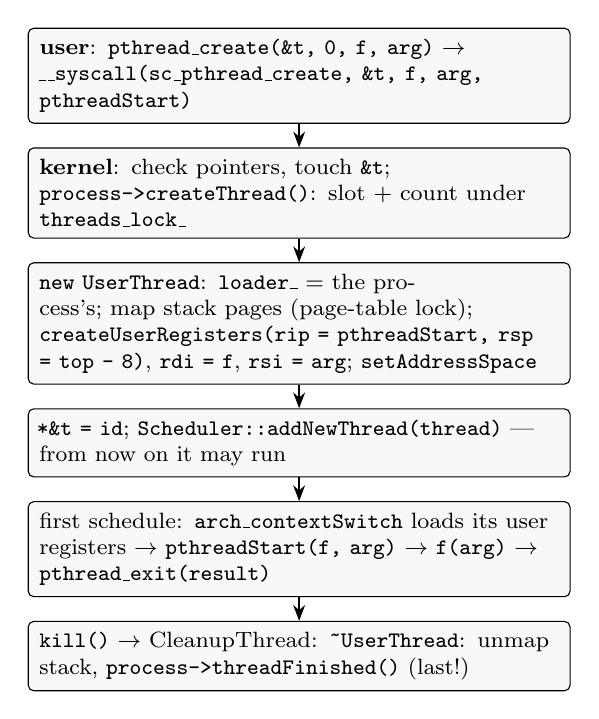
\begin{tikzpicture}[
  box/.style={draw, rounded corners=2pt, fill=codebg, align=left, font=\footnotesize,
              inner sep=4pt, text width=6.6cm},
  arr/.style={-{Stealth[length=2mm]}, thick}]
  \node[box] (a) {\textbf{user}: \code{pthread\_create(\&t, 0, f, arg)} $\to$
     \code{\_\_syscall(sc\_pthread\_create, \&t, f, arg, pthreadStart)}};
  \node[box, below=3mm of a] (b) {\textbf{kernel}: check pointers, touch \code{\&t};
     \code{process->createThread()}: slot + count under \code{threads\_lock\_}};
  \node[box, below=3mm of b] (c) {\code{new UserThread}: \code{loader\_} = the process's;
     map stack pages (page-table lock); \code{createUserRegisters(rip = pthreadStart,
     rsp = top - 8)}, \code{rdi = f}, \code{rsi = arg}; \code{setAddressSpace}};
  \node[box, below=3mm of c] (d) {\code{*\&t = id}; \code{Scheduler::addNewThread(thread)} --- from now on it may run};
  \node[box, below=3mm of d] (e) {first schedule: \code{arch\_contextSwitch} loads its user registers
     $\to$ \code{pthreadStart(f, arg)} $\to$ \code{f(arg)} $\to$ \code{pthread\_exit(result)}};
  \node[box, below=3mm of e] (f) {\code{kill()} $\to$ CleanupThread: \code{\textasciitilde UserThread}: unmap stack,
     \code{process->threadFinished()} (last!)};
  \draw[arr] (a) -- (b); \draw[arr] (b) -- (c); \draw[arr] (c) -- (d); \draw[arr] (d) -- (e); \draw[arr] (e) -- (f);
\end{tikzpicture}
\end{center}

\section{Tutorial 1: a string from user space}
\label{sec:tutorial1}

The first A0 tutorial --- reproduced unchanged in ex11 --- added a syscall that copies a user
string (at most 15 characters) into a \code{ustl::string s} member of the calling thread,
under a per-thread \code{Mutex s\_mutex} (\code{ScopeLock}), with a debug flag of its own:

\begin{lstlisting}[style=cpp]
const size_t TUTORIAL = Ansi_Blue | OUTPUT_ENABLED;      // debug.h: one line per flag

    case sc_tutorial:
      tutorial((char*)arg1);                             // the result is dropped!
      break;
\end{lstlisting}

\textbf{What a tutor would ask about it} (all fixed in A0-11):
\begin{itemize}
\item the \code{case} has no \code{return\_value =} --- every call returns 0, also for \code{NULL};
  and \code{return -1U} is \code{0xFFFFFFFF}, not -1;
\item only the \emph{first} byte is checked against \code{USER\_BREAK}: a string without NUL
  right below it makes \code{strncpy} read \code{0x800000000000} $\to$ General Protection Fault in
  the kernel, the process is killed (exit 888). A string's end is unknown: copy byte by byte,
  check each address before reading it;
\item \code{strncpy(temp, string, 15)} leaves \code{temp} without NUL for long strings --- write
  it yourself;
\item \code{debug(TUTORIAL, "\%s", string)} prints the \emph{user} string again: a second,
  unbounded read after the copy --- print the copy;
\item the per-thread Mutex: needed only if another thread or kernel path touches the field.
  Be ready to say which accesses a lock orders --- and when none does.
\end{itemize}

\section{Tutorial 2: one page at two addresses}
\label{sec:tutorial2}

The second A0 tutorial (7 Oct) added two syscalls --- reproduced unchanged in ex12:

\begin{lstlisting}[style=cpp]
size_t Syscall::get_physical_address(size_t virtual_address)
{
  UserProcess *process = (UserProcess*)currentThread;
  ArchMemoryMapping m = process->loader_->arch_memory_.resolveMapping(virtual_address >> 12);
  return m.page_ppn;
}
void Syscall::map_address(size_t virtual_address, size_t ppn)
{
  UserProcess *process = (UserProcess*)currentThread;
  bool mapped = process->loader_->arch_memory_.mapPage(virtual_address >> 12, ppn, 1);
  assert(mapped);
}
\end{lstlisting}

The user program asks for the frame of a global, maps it at \code{0x424242424242}'s page, and
reaches the global through \code{(vpn << 12) + (\&global \& 0xfff)}: the page table translates
only the page number, the 12-bit offset is the same in the virtual and the physical address.

\textbf{Why it panics at exit.} \code{exit} $\to$ \code{kill} $\to$ CleanupThread $\to$
\code{\textasciitilde UserProcess} $\to$ \code{\textasciitilde Loader} $\to$
\code{\textasciitilde ArchMemory}, which frees \emph{every} present user page. The global's frame is
present twice $\to$ \code{freePPN} twice $\to$ \code{Assertion "Double free PPN"}. The program
itself had finished correctly; the backtrace names the CleanupThread.

\textbf{What a tutor would ask about it} (all fixed in A0-12):
\begin{itemize}
\item any \code{ppn} is accepted --- a process can map another process's frame or the kernel's
  code, writable. Only frames already mapped in the caller's own address space (walk the user
  half like \code{\textasciitilde ArchMemory}; there is no reverse map);
\item no \code{USER\_BREAK} check, and \code{assert(mapped)}: a user program crashes the kernel by
  mapping an address that is in use --- return \code{-1}, asserts are for kernel bugs;
\item \code{page\_ppn} of an unmapped page is 0, a real frame number --- check
  \code{m.page\_size == PAGE\_SIZE}, else \code{-1} (an untouched page is unmapped: lazy loading);
\item no page-table lock (ex02) --- needed as soon as a process has threads;
\item the double free: remember the alias vpns, unmap them with \code{unmapPage(vpn, false)} in
  \code{Loader::\textasciitilde Loader} --- which runs before \code{arch\_memory\_} is destroyed;
\item \code{(UserProcess*)currentThread}: not needed in base SWEB, wrong in the team repo
  (\code{getLoader()}).
\end{itemize}
No TLB flush is needed after \code{mapPage}: the entry was not present before.

\section{Variants to expect}

Practise these as ``five-minute variations'' of the tasks:
\begin{itemize}
\item \code{mmap}-like: map \code{n} pages at an address chosen by the kernel / by the user
  (A0-02 with a length); \code{munmap} with partial ranges.
\item the page fault handler counts faults per process; a syscall returns the count.
\item a special address that does something else: returns the time, the tid, a page shared by
  all processes (careful: \code{unmapPage} frees the page --- shared pages need a reference count).
\item tutorial-2 style: the physical page of an address; map a frame of the process a second
  time; ``give me a second address for this variable'' --- remember: a frame mapped twice is
  freed twice at exit (\S\ref{sec:tutorial2}).
\item ``when a process writes to page X, print a message and continue'' (map it on demand,
  read-only first, then writable on the write fault).
\item the segv handler for division by zero (\code{errorHandler}); with a second argument
  (read/write); resumable (needs a sigreturn syscall).
\item \code{pthread\_create} variants: thread starts with two arguments; a thread that runs a
  function \code{n} times; \code{pthread\_multi} with one thread \emph{per} function.
\end{itemize}

\chapter{A1: threads, scheduling, processes}
\label{ch:a1}

The A1 tasks students reported fall into five families. All of them build on the same few
mechanisms: \emph{where} a thread's state lives, \emph{who} frees it \emph{when}, and
\emph{how} threads wait for each other. In the course, A1-01 (\code{pthread\_join}) builds that
base on top of A0-08; in the interview it is your team's implementation.

\section{The thread bookkeeping every A1 task needs}

\begin{center}
\small
\begin{tabular}{L{4cm}L{10.8cm}}
\toprule
\textbf{Question} & \textbf{Course solution (base SWEB) --- find the equivalent in your team repo} \\
\midrule
Which threads does a process have? & \code{UserProcess::slots\_[]}: state FREE / RUNNING / FINISHED, id, exit value, \code{UserThread*} (valid while RUNNING) \\
Which lock? & \code{UserProcess::threads\_lock\_} (Mutex) for all of it; \code{threads\_changed\_} (Condition), broadcast whenever a thread finishes \\
Where does the exit value survive the thread? & in the slot --- the thread object is deleted by the CleanupThread at an unknown time \\
When is a thread object freed? & by the CleanupThread, after \code{kill()}; its destructor unmaps the stack and calls \code{threadFinished()} \emph{as its last action} \\
How do I use another thread safely? & \code{findThread(id)} under \code{threads\_lock\_}, use the pointer only while holding it: the object is freed only after \code{threadFinished}, which needs that lock \\
When is a slot reused? & after \code{pthread\_join} (FINISHED $\to$ FREE), never earlier \\
\bottomrule
\end{tabular}
\end{center}

\begin{lockbox}
\begin{itemize}
\item One Mutex for the per-process thread table, one Condition, \textbf{broadcast}: different
  waiters wait for different things (join of thread 3, join of thread 5, exit waiting for all).
\item After every \code{wait()}, re-check \emph{your} condition including identity (the slot may
  have been joined by someone else and reused).
\item Never create a thread object (which allocates and takes the page-table lock) while holding
  the thread table lock --- no nested locks if you can avoid them.
\item Never \code{kill()} a thread while it holds a lock --- not even itself.
\end{itemize}
\end{lockbox}

\section{Family 1: creating and waiting (join, multiple, join\_any, barriers)}

\begin{description}
\item[Create] = shared address space + own stack + own registers + \code{addNewThread}
  (A0-08). \emph{All or nothing} (\code{pthread\_multiple}): create every object first,
  schedule only when all exist; a never-scheduled thread may be deleted directly.
\item[Wait] = Mutex + Condition + state, \code{while} loop. Join waits for FINISHED,
  \code{join\_any} for ``any of these FINISHED, or none alive any more'' (then fail instead of
  waiting forever), barriers for ``my round's generation changed'' --- \emph{not} for a counter that
  the next round changes again.
\end{description}

\section{Family 2: the scheduler (flagging, invoke, switch, runtime)}

\code{Scheduler::schedule()} (\file{common/source/kernel/Scheduler.cpp}) runs in the timer
interrupt and in \code{yield}'s interrupt: \textbf{interrupts are off, no lock can be taken}.
It walks \code{threads\_}, picks the first \code{schedulable()} one and rotates the list.

\begin{itemize}
\item Data the scheduler reads must be single words written atomically (\code{ArchThreads::atomic\_set}):
  a ``run twice'' flag (A1-04), a ``run this one next'' pointer (A1-05), a per-thread tick
  counter written in \code{incTicks} (A1-07).
\item A pointer handed to the scheduler may dangle by the time it runs: only use it after finding
  it in \code{threads\_} (every list member is alive).
\item The timer runs at 18.2\,Hz (\code{IRQ0\_TIMER\_FREQUENCY} 0 $\to$ PIT divisor 65536): one tick
  is 55\,ms. A \code{sched\_yield} round passes the IdleThread, which halts until the next tick ---
  so \textbf{every yield can cost a whole tick}. Tests (and your solutions) should sleep on a
  Condition rather than yield in loops.
\end{itemize}

\section{Family 3: ending threads (exit, cancel)}

\begin{itemize}
\item \textbf{exit} (POSIX): the whole process ends. Base SWEB: the main thread waits for the others
  (A0-08 simplification). Your team: all threads must be stopped --- \emph{from outside}, which is
  the same problem as cancel.
\item \textbf{cancel} (deferred, A1-06): set a flag; the target dies at its next cancellation point
  (syscall entry, while waiting in join --- wake it with a broadcast), never in the middle of a
  syscall holding locks. A thread that never makes a syscall keeps running.
\item The exit value: \code{PTHREAD\_CANCELED} (-1) for a cancelled thread, -1 for one killed by a fault.
\end{itemize}

\section{Family 4: registers and stacks (snapshot/revive, upcalls, 15 arguments)}

\code{user\_registers\_} during a syscall is the state the thread continues with (\S\ref{sec:registers}).
Snapshot/revive (A1-08) restores \emph{registers and the used part of the stack}: registers alone point
into frames that have been overwritten since. Copy \code{ArchThreadRegisters} field by field (its
\code{fpu} pointer and destructor make struct copies dangerous). More than 5 syscall arguments: pass a
pointer to an array and copy it in once.

\section{Family 5: memory and processes (vtop/ptov, shm, sbrk, page fault statistics)}

\begin{itemize}
\item \code{resolveMapping} answers virtual $\to$ physical; physical $\to$ virtual needs a walk of
  the page tables (no reverse map in SWEB).
\item A page in two address spaces needs a \textbf{reference count} and an unmap that does not free;
  process exit (\code{\textasciitilde ArchMemory} frees every present page!) must drop references
  first --- in \code{\textasciitilde Loader}, before the member \code{arch\_memory\_} dies.
\item The page-fault C entry \code{pageFaultHandler(address, error)} runs with interrupts off: atomics
  only. \code{cr2} is read by the assembly stub immediately, because the next fault overwrites it.
\end{itemize}

\section{Not in the course, and how you would do it}

\begin{description}
\item[forkall] Fork with every thread: copy the page tables (or COW), then for every thread of the
  parent create a thread in the child with a copy of its user registers and the same stack slot
  (\code{rax} = 0 for the caller). Hold the parent's page-table lock while copying. The design
  question a tutor will ask: what about a parent thread that is \emph{inside a syscall} right now
  (e.g.\ sleeping in \code{pthread\_join})? Its \code{user\_registers\_} hold its state at syscall
  entry --- the child's copy would continue after a syscall it never finished. Options: give the copy
  the result -1, or stop all threads at the user/kernel boundary first (like cancel's safe points).
\item[special address in the page fault handler] A0-04, with a different action: kill only the
  faulting thread, print all threads' registers (\code{ArchThreads::printThreadRegisters}).
\item[pthread\_switch] A directed yield (A1-05) where the caller additionally sleeps until someone
  switches back to it: \code{Scheduler::sleep()} after setting the preferred thread --- careful
  with lost wake-ups (the target may switch back before you sleep): use a Condition with a state.
\end{description}

\chapter{A2: swapping, copy-on-write, page-table bits}
\label{ch:a2}

A2 tasks change what a page-table entry means and where a page's content lives. Three ideas
carry all of them: \textbf{a non-present entry can carry information}, \textbf{take the page
away before you touch its content}, and \textbf{a physical page may have more than one owner}.

\section{A page-table entry, three meanings}

\begin{center}
\small
\begin{tabular}{L{3.6cm}L{4.4cm}L{6.8cm}}
\toprule
\textbf{State} & \textbf{Bits} & \textbf{Meaning} \\
\midrule
not mapped & all zero & no page here (lazy: \code{loadPage} on the first access) \\
present & \code{present = 1}, \code{page\_ppn} = frame & normal; \code{writeable}, NX, \code{dirty}, \code{accessed} apply \\
swapped out (A2-01) & \code{present = 0}, marker in \code{ignored\_2}, \code{page\_ppn} = slot & the CPU ignores all bits of a non-present entry --- they are yours \\
present + clean copy (A2-05) & \code{present = 1}, \code{ignored\_1} = slot + 1 & content also on disk; \code{dirty} tells whether it is still equal \\
shared zero page (A2-09) & \code{present = 1}, \code{writeable = 0}, \code{page\_ppn} = zero page & the first write copies \\
\bottomrule
\end{tabular}
\end{center}

\begin{trapbox}
\code{ArchMemory::unmapPage} frees a page table as soon as no entry in it is \emph{present}. With
swapped entries that is wrong: it would throw away the slot numbers. Treat ``all entries zero'' as
empty (A2-01). Likewise \code{\textasciitilde ArchMemory} frees every \emph{present} page: shared
pages (A1-10) and the zero page (A2-09) must be excluded, swap slots (A2-01) freed separately.
\end{trapbox}

\section{Swap out and in --- the order is the whole task}

\begin{center}
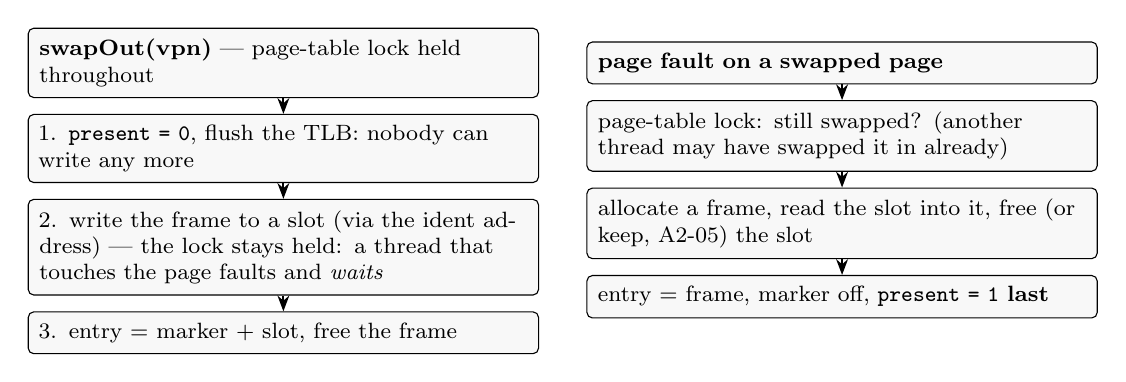
\begin{tikzpicture}[
  box/.style={draw, rounded corners=2pt, fill=codebg, align=left, font=\footnotesize,
              inner sep=4pt, text width=6.2cm},
  arr/.style={-{Stealth[length=2mm]}, thick}]
  \node[box] (a) {\textbf{swapOut(vpn)} --- page-table lock held throughout};
  \node[box, below=2mm of a] (b) {1. \code{present = 0}, flush the TLB: nobody can write any more};
  \node[box, below=2mm of b] (c) {2. write the frame to a slot (via the ident address) --- the lock stays held:
     a thread that touches the page faults and \emph{waits}};
  \node[box, below=2mm of c] (d) {3. entry = marker + slot, free the frame};
  \draw[arr] (a) -- (b); \draw[arr] (b) -- (c); \draw[arr] (c) -- (d);
  \node[box, right=6mm of a] (e) {\textbf{page fault on a swapped page}};
  \node[box, below=2mm of e] (f) {page-table lock: still swapped? (another thread may have swapped it in already)};
  \node[box, below=2mm of f] (g) {allocate a frame, read the slot into it, free (or keep, A2-05) the slot};
  \node[box, below=2mm of g] (h) {entry = frame, marker off, \code{present = 1} \textbf{last}};
  \draw[arr] (e) -- (f); \draw[arr] (f) -- (g); \draw[arr] (g) -- (h);
\end{tikzpicture}
\end{center}

\begin{lockbox}
\begin{itemize}
\item \textbf{Disk I/O while holding the page-table Mutex is allowed} --- and here it is what keeps
  other threads off the half-written page. A SpinLock would be wrong: the request sleeps.
\item One lock order for all of A2: page-table lock $\to$ PageManager $\to$ swap bookkeeping
  (\code{SwapManager}). Your team's swap thread must use the same order.
\item Read the \code{dirty} bit only after \code{present = 0} + flush --- before that a write can still set it.
\item Removing rights (present, writable, NX) $\Rightarrow$ TLB flush in the critical section.
  Changing the frame of a present mapping (COW, relocation) $\Rightarrow$ flush.
\end{itemize}
\end{lockbox}

\section{The swap device}

\code{idea2} is a 50\,MiB partition of type 0x82 that base SWEB never uses:
\begin{lstlisting}[style=cpp]
BDVirtualDevice* swap = BDManager::getInstance()->getDeviceByName("idea2");
\end{lstlisting} Slot $s$ = bytes
$[s \cdot 4096, (s+1) \cdot 4096)$, written and read through the frame's ident address
(\code{readData}/\code{writeData}, ex08). Create the bookkeeping object in \code{startup()} after
\code{BDManager::doDeviceDetection()}; do disk I/O only from threads (the request yields until the
IDE interrupt) --- \code{startup()} itself is too early (A2-11 reads its record in
\code{ProcessRegistry::Run()}). \code{run\_test.sh} boots with a throw-away disk; \code{--keep-disk}
keeps one copy over several boots.

\section{Copy-on-write}

A write to a present read-only page faults with \code{present = 1, writing = 1} --- such faults are
rejected by \code{checkPageFaultIsValid}, so the COW branch goes \emph{before} it. CR0.WP is set
(\code{boot.32.C}), so the \textbf{kernel's} writes into user memory fault as well: a COW branch that
requires \code{user} breaks every syscall that writes into a fresh buffer. The copy is
\code{allocPPN} + \code{memcpy} between ident addresses; the zero-page case (A2-09) needs no
\code{memcpy}. Fork's COW (your mandatory part) adds reference counts per frame and two processes'
page tables --- lock both in a fixed order (e.g.\ by address) or copy the entries under the parent's
lock only.

\section{Moving pages behind a process's back}

Swap-out, relocation (A2-10), defragmentation, ``swap out all pages'' (F3): the process may run at any
moment (preemption!) and touch the page. The pattern is always the same: \emph{present = 0 first,
work, present = 1 last}, under the page-table lock; and the page-fault handler, finding a non-present
page, must first take that lock and check whether the page is back --- \emph{before} treating it as a
new page (\code{loadPage} would kill the process for a stack page). A thread that works on
\emph{other} processes' memory needs a list of address spaces with its own lock, taken
\emph{before} any page-table lock, and must keep each process alive while it works on it.

\section{Sketches for the tasks not in the course}

\begin{description}
\item[Defragmentation (F7)] Walk all swapped entries of all processes (list of address spaces as in
  A2-10), move slot contents so the used slots are contiguous, update each entry --- under each
  process' page-table lock, one slot at a time; the slot bitmap under its own lock.
\item[Deduplication of arbitrary pages] Hash present pages (a kernel thread), compare equal hashes
  byte by byte, map one frame read-only into both with a reference count, COW on write (A2-09).
\item[mmap a file] A region per process; the page fault reads the file part through
  \code{VfsSyscall::read} (like \code{Loader::readFromBinary}); \code{msync}/\code{munmap} write dirty pages back.
\item[ASLR] Randomise the stack top in \code{UserProcess} (and the heap start) with \code{rdtsc};
  the code segment needs position-independent binaries.
\item[Checksum check] Keep a checksum per swapped page (in a table or in the entry's free bits),
  verify after swap-in, kill the process (or panic) on mismatch.
\item[Unswappable pages / pages of the own process may not be swapped] A flag in the entry's free
  bits that the swap policy checks; \code{mlock}-like syscall to set it.
\end{description}

\chapter{Base SWEB vs.\ your team repo}
\label{ch:team}

The interview happens in \textbf{your group's repository}, not in base SWEB. Since Phase 0 it
separates process and thread. The mechanisms are identical; some names and the place for
per-process state differ. State of \code{osw26e3} \code{main} on 6 Oct 2026 --- check again
before the interview, the team keeps changing it.

\begin{center}
\small
\begin{tabular}{L{6.4cm}L{8.4cm}}
\toprule
\textbf{Base SWEB / this course} & \textbf{Team repo (osw26e3)} \\
\midrule
\code{class UserProcess : public Thread} (the process \emph{is} its only thread) &
\code{class UserProcess} (no thread), \code{class UserThread : public Thread}, \code{createMainThread()} \\
\code{currentThread->loader\_} & \code{currentThread->getLoader()} (the loader belongs to the process) \\
\code{currentThread->process\_} (added in A0-08) & \code{currentThread->getProcess()} (\code{Thread::process\_}) \\
per-process state in \code{Loader} (\code{heap\_size\_}, segv handler, \ldots) & per-process state in \code{UserProcess} \\
\code{Loader::arch\_memory\_lock\_} (added by this course) & whatever lock your team uses for the page tables --- \textbf{find it before the interview}; if there is none, that is the first thing a tutor asks about \\
\code{UserProcess::createThread} (A0-08) & your team's \code{pthread\_create} (P1) --- know its steps \\
syscall numbers 1400--1799 & your own block (1500--1999) --- avoid collisions with the team's syscalls \\
\code{process\_->waitForThreads()} in \code{exit} & your team's exit/join design \\
\bottomrule
\end{tabular}
\end{center}

\begin{infobox}[title=\textbf{Before the interview: 15 minutes in the team repo}]
\begin{enumerate}
\item Where is the page-table lock? Which locks does \code{UserProcess} have, what do they protect?
\item Where does \code{pthread\_create} map the stack, set the registers, add the thread?
\item Where are a process's threads listed, and who frees the address space when?
\item Add a trivial syscall in a scratch branch and run it --- so the six places are fresh.
\end{enumerate}
\end{infobox}


\end{document}
